\chapter{Related Work}\label{ch:rel}
\section{Text Classification}

Text Classification is a common supervised learning task in which a body of text, or document containing text, needs to be assigned to a set of class labels. Common applications of text categorization include article categorization, spam detection, sentiment analysis, and authorship attribution \cite{Sebastiani2002, Croft, Shrestha}. Pivotal work in this area includes Joachim’s approach that utilized Support Vector Machines (SVMs), which has remained influential \cite{Joachims1998}. Apart from SVMs, multinomial- and Bernouilli-kernelled Naive Bayes (NB), and Logistic Regression are often utilized for these problems \cite{Croft, Wang2012}. However, in order to enable algorithms to take advantage of the information represented by words, we first need to create a representation of text that algorithms can work with. Common feature-generating methods such as the Bag-of-Words (BoW) model, ngrams, the term frequency-inverse document frequency (tf-idf), and word vectors have been used with great effect \cite{Manning2008}.\\
\\
In the BoW model, originally introduced by Harris \cite{Harris1954} every word gets represented by an index in a vector, which can thus grow incredibly spare with the vocabulary used. A sentence of natural language is then simply represented by a sparse vector containing counts of each word appearing in the vocabulary. A problem is that this vocabulary grows larger the more unique words appear in a text.\\ 
\\
On a conceptual level, ngrams are similar to the BoW approach and can be either applied to words or individual characters. The idea is, to look at adjacent words and take counts of words appearing next to each other, instead of focusing on singular words. For instance, a n-gram approach involving bigrams (2-grams) takes two words together, and produces a feature vector that represents a sentence by these counts. A sliding window approach is used to move across a sentence. Both BoW and ngrams are relatively naive methods of dealing with text, as all words or ngrams are considered to be equally important. \\
\\
The tf-idf weighting method tries to address this problem by multiplying a how often a term appears in a document with a log function of how many documents there are in the collection divided by how many document contain the term. If a word is common across all documents this assigns a lower weight than words that are rare across all documents, meaning that rarer words which are theorized to contribute more to the meaning of a document contribute more. The formula for tf-idf is shown below, where tf is the term frequency of term t in document d, N is the total number of documents in the corpus, and df is the document frequency of term t.
\\
\begin{center}
	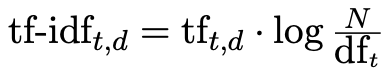
\includegraphics[width=0.35\textwidth]{tf-idf.png}
\end{center}

This has a shortfall in that we still treat words as simply random-ordered features present in a document. Indeed, speakers of natural language will know that word order is actually very important and yet this information is simply lost when converting text to an tf-idf feature vector because it loses the order in which words appear.\\
\\
A different take on word vector representations comes from word embed- dings, popularized by methods such as word2vec \cite{Mikolov2013}. Word embeddings are a representation of a word as a single vector, and the idea has in fact been around for longer \cite{Bengio2003}. These vector space methods often involve a shallow neural network to produce word embeddings learned from processing large amounts of data \cite{Mikolov2013, Levy2014, Goldberg2016}. Commonly, these are 50 to 300-dimensional vectors, although more recent work incorporates much higher dimensionality [\cite{Devlin2018, Peters2018}. As Word2vec was one of the first such methods to become popular, it has been well-studied as a result. The appeal and relative simplicity means it can readily be used for classification, recommendation, and similarity matching \cite{Kenter2015}. Word embedding methods quickly became a state-of-the- art staple in text classification \cite{Peters2018, Howard2018}. However, for classical methods such as SVMs, it appears that using word embeddings decreases performance \cite{Lilleberg2015}.\\
\\
A lot of work has been done to evaluate word embeddings as well to develop new embedding approaches. There many adaptions and similar methods available such as doc2vec \cite{Le2014}, syntax-aware wang2vec \cite{Ling2015}, fastText \cite{Bojanowski2016}, and Stanford’s log bi-linear Glove, which does not rely on a shallow neural network \cite{Pennington2014}.
A key idea is that these embeddings can be learned on data outside the target data set. This is an elegant way to take information from a corpus such as, for instance, a Wikipedia dump and use it to collect contextual information on word occurrences, which can then be applied to, for instance, a sentiment analysis task based on the short text gathered from internet comments. However, the word embeddings learned from data will carry any implicit biases present in their training texts [6], although one could argue this is exactly the type of similarities we intend to capture in the harmonized system text domain. It remains hard to apply word embeddings to scenarios where training data is limited or consisting of short messages. In this line, work has been done to increase performance with data from another domain \cite{Abdelwahab2016}.


\section{Short Text Classification}

A specific sub-field of text categorization deals with short text. Short text is especially prevalent online, where it can take the form of twitter messages, reviews, titles, chat messages, URLs, and search queries. Due to the limited information contained in a message the problem is characterized by data sparsity and a lack of context \cite{Wang2017}. This is especially true with regards to Twitter messages (also known as Tweets) and chat messages, which are often limited in the amount of characters or words in a sentence. Recurring problems are also that these texts do not usually follow natural language conventions: in order to stay brief, these texts often contain a telegram-style syntax and common natural language processing techniques do not apply in the same way they do with spoken text, or longer text as is common in books. This results in a problem of ambiguity, where a piece of text might have multiple meanings but does not provide enough context to figure out which meaning was intended. Often, these texts also include specific tokens and characters unique to the domain. Interestingly, it has been shown that Naive Bayes models outperform SVMs if the text length is limited, while for longer text the opposite still holds true \cite{Wang2012}.

\section{Neural Network for Text}
Neural networks for natural language processing have experienced a surge in popularity in recent years. The most common methods can be roughly grouped in two categories: Convolutional Neural Networks (which includes the approach in this thesis) and Recurrent Neural Networks (which include Long-Short-Term Memory (LSTM) networks and Gated Recurrent Units (GRUs)).\\
\\
Recurrent neural networks are not an odd choice, as they excel with modelling sequential data. They have been utilized for language model problems and have in general been applied with success \cite{Mikolov2010a, Chung2014, Lai2015, Howard2018, Xu}. However, they were initially not well-suited to deal with correlations that are further apart in sentences, due to the vanishing gradient problem during back- propagation where the gradient propagated through the network becomes close to zero when more time steps are made.\\ 
\\
With word embeddings, neural networks for text gained a significant boost in popularity and researchers such as Kim \cite{Kim2014} and Kalchbrenner\cite{Kalchbrenner2014} soon released their work with feed-forward one-dimensional convolutional neural networks based on word embeddings. The general architecture is much simpler than the convolutional neural networks used in computer vision, as the architectures used often consist of just an embedding layer, a convolutional layer, a max-pooling layer and a varying amount of dense layers for each of a set of pre-defined filter sizes. Interestingly, this shallow and wide architecture remains a impressive baseline \cite{Le2017}. The idea behind the convolutional layers’ is that this is akin to taking ngrams with varying convolutional filter sizes \cite{Zhang2015, Jacovi2018} . Pooling strategies have been shown to help, as they eliminate poorer ngrams and bring down the training complexity of the network; however, others opt out of pooling completely [\cite{Kim2014, Zhang2015}. Some architectures use multiple filter sizes in a multi-channel approach \cite{Kim2014,Liu2017,Goldberg2016}.\\
\\
Current approaches also include bi-directional LSTMs, which pass over text both from left-to-right \cite{Radford2018} and right-to-left. This greatly enhances the ability of RNNs to deal with longer dependencies in text. Among these, the ELMo model \cite{Peters2018} successfully applies this concept to produce embeddings that change on differing sentences (context).\\ 


\section{Google BERT}
Attention mechanisms are also popular and are currently popular choices to capture dependencies in text \cite{Lin2017, Openai}. One specific attention mechanism is the transformer, an encoder-decoder architecture that involves an attention mechanism to capture dependencies in text \cite{Vaswani2017}. BERT (Bidirectional Encoder Representations from Transformers) \cite{Devlin2018} successfully combines this idea with a Masked Language Model objective to produce a complex language model that can be applied to many downstream tasks. It is worth noting that the concept of pre-training on outside data and applying a trained model to supervised tasks is still adhered to with these models. However, with these developments it seems that the concept of transfer learning in language models is definitely shifting from mere word embeddings to more sophisticated models that have been trained for a long period of time, which is very much like the trend in computer vision.\\
\\
BERT’s \cite{Devlin2018} (Bidirectional Encoder Representations from Transformers) key technical innovation is applying the bidirectional training of Transformer \cite{Vaswani2017}, a popular attention model, to language modelling. This is a new approach to NLP field which looked at a text sequence either from left to right or combined left-to-right and right-to-left training. The paper’s show that a trained bidirectional language model can have a deeper sense of language context and flow rather than single-direction language models. Researchers also detailed a new technique named MLM (Masked LM) which allows to train bidirectional models which was previously impossible. \\
The model is also pre-trained on two unsupervised tasks, masked language modeling and next sentence prediction. This allows the use of pre-trained BERT model by fine-tuning the same on downstream specific tasks such as sentiment classification, text classification, question answering and more.\\
\\
In addition to all of that, Google BERT, is the current new standard in NLP algorithm, since he was presented, it has been the new based of many new NLP algorithm such as Facebook RoBERTa \cite{Liu2019d}, XLNet \cite{Yang2019}, Nvidia Megatron \cite{Shoeybi} for exemple. Bert is also mention in other paper \cite{Zhu2019, Wang2019c}. \\ 
\\
Recently Google made a new breakthrough in the NLP field first with ALBERT (A Lite BERT for Self-supervised Learning of Language Representations) \cite{Lan} and a month later with T5\cite{Raffel2019}. ALBERT is using BERT as a based of the new model by tweaking it to make BERT as a lite version and taking off some parameters that are judges as inefficient such as the Next Sentence Prediction (NSP).

\subsection{How Google BERT works ?}
As previously say, BERT,  makes use of Transformer  \cite{Vaswani2017}, an attention mechanism that learns contextual relations between words (or sub-words) in a text. In its vanilla form, Transformer includes two separate mechanisms : 

\begin{itemize}
\item an encoder that reads the text input.
\item a decoder that produces a prediction for the task
\end{itemize}

Since BERT’s goal is to generate a language model, only the encoder mechanism is necessary. This detailed are described in the paper made by Google researchers \citeauthor{Devlin2018} \cite{Devlin2018}. \\
\\
As opposed to directional models, which read the text input sequentially (left-to-right or right-to-left), the Transformer encoder reads the entire sequence of words at once. Therefore it is considered bidirectional. This characteristic allows the model to learn the context of a word based on all of its surroundings (left and right of the word).\\
\\
The figure 2.1 below is a high-level representation of the Transformer encoder. The input is a sequence of tokens, which are first embedded into vectors and then processed in the neural network. The output is a sequence of vectors of size H, in which each vector corresponds to an input token with the same index. \\
\\
Unlike \citeauthor{Peters2018} and \citeauthor{Radford2018}, Google researchers are not using traditional left-to-right or right-to-left language models to pre-train BERT. Instead, they pre-train BERT using two unsupervised tasks, described bellow:

\begin{itemize}
\item Masked Language Model (MLM)
\item Next Sentence Prediction (NSP)
\end{itemize}

\subsection{Masked Language Model}
Before feeding word sequences into BERT, 15{\%} of the words in each sequence are replaced with a [MASK] token. The model then attempts to predict the original value of the masked words, based on the context provided by the other, non-masked, words in the sequence. In technical terms, the prediction of the output words requires:
\begin{itemize}
\item Adding a classification layer on top of the encoder output.
\item Multiplying the output vectors by the embedding matrix, transforming them into the vocabulary dimension.
\item Calculating the probability of each word in the vocabulary with softmax.
\end{itemize}

\begin{figure}[h]
\centering
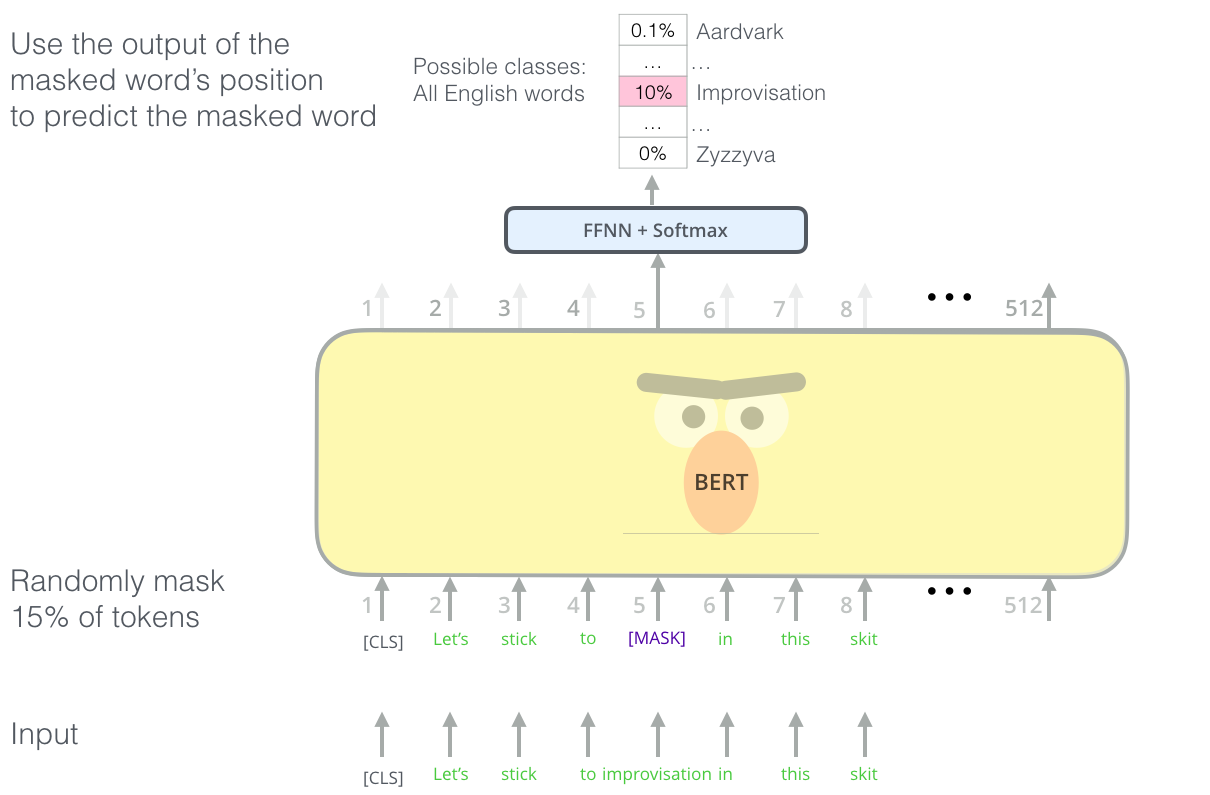
\includegraphics[width=1\textwidth]{BERT-language-modeling-masked-lm.png}
\caption{BERT's clever language modeling task masks 15{\%} of words in the input and asks the model to predict the missing word. \url{https://jalammar.github.io/illustrated-bert/}}
\label{fig:MLM}
\end{figure}

\clearpage
\subsection{Next Sentence Prediction}
During the pre-training phase, the model receives in input a pairs of sentences and learn how to predict if the second sentence is the actual next sentence of the original document. Half of the inputs is predicted as the actual next sentence while the other half is predicted as a random sentence from the corpus.\\
\\
According to the researchers, in order to help the model distinguish between the two inputs sentences, the input is processed as follows before entering the model:
\begin{itemize}

    \item A [CLS] token is inserted at the beginning of the first sentence and a [SEP] token is inserted at the end of each sentence.
    \item A sentence embedding indicating Sentence A or Sentence B is added to each token. Sentence embeddings are similar in concept to token embeddings with a vocabulary of 2.
    \item A positional embedding is added to each token to indicate its position in the sequence. The concept and implementation of positional embedding are presented in the Transformer paper.
\end{itemize}

\begin{figure}[h]
    \centering
    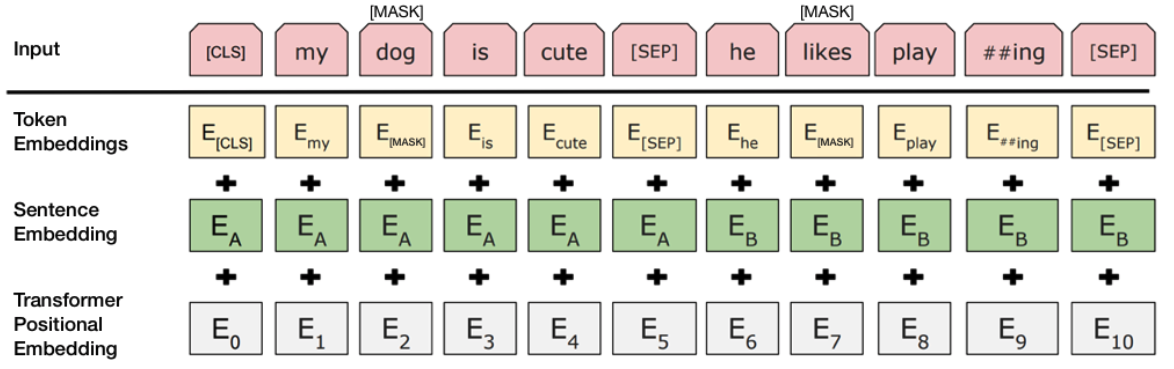
\includegraphics[width=1\textwidth]{NSP.png}
    \caption{BERT \cite{Devlin2018} input representation. The input embeddings are the sum of the token embeddings, the segmentation embeddings and the position embeddings.}
    \label{fig:NSP1}
\end{figure}

\begin{figure}[h]
    \centering
    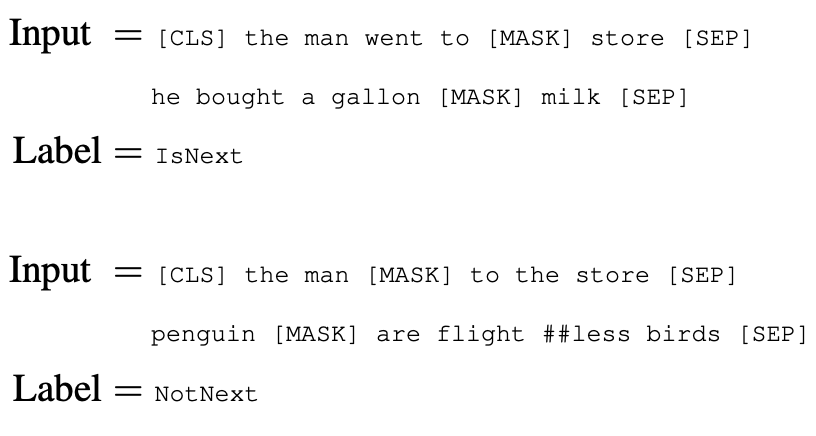
\includegraphics[width=0.8\textwidth]{NSP2.png}
    \caption{The next sentence prediction can be illustrated as following exemples \cite{Devlin2018}}
    \label{fig:NSP2}
\end{figure}

\clearpage
\subsection{Fine Tuning}
Thanks to the pre-training steps describe above, fine-tuning BERT is kind of straightforward. \\
As describe in section 3.2 of \citeauthor{Devlin2018}, BERT can be used for a wide variety of NLP tasks, as shown in the figure below.

\begin{figure}[!h]
    \centering
    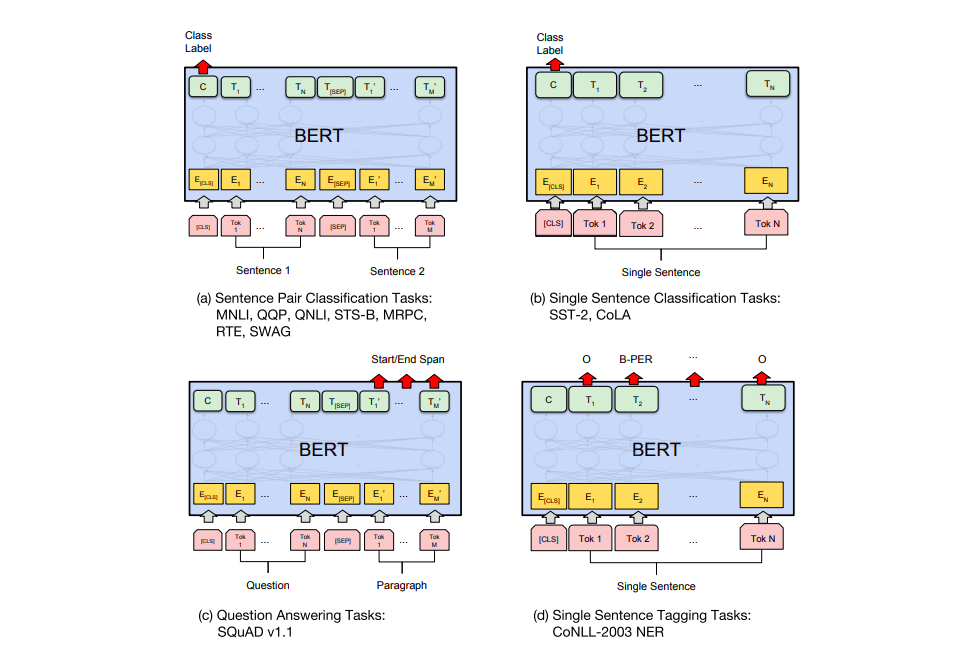
\includegraphics[width=1\textwidth]{bert-tasks.png}
    \caption{Illustrations of Fine-tuning BERT on different tasks, appendix B of \cite{Devlin2018}}
    \label{fig:Fine-tuning}
\end{figure}

In this thesis, We will use the the top right fine-tuning process "Single Sentence Classification" as it is the most suitable to the methods described in chapter 4.\\
\\
This section described two mains key components of Google BERT, the first one was the pre-training process with the Masked Language Model and the Next Sentence Prediction. 
The second one was the fine tuning phase. Due to his conception, BERT can be easily fine-tune, and therefore it mainly less expensive than do the pre-training phase. 
According to the paper every result can be replicated in at most 1 hour with a Cloud TPU or a few hours on a GPU starting with the exact same pre-train model. 
All model are available on the GitHub\footnote{\url{https://github.com/google-research/bert}} repository  or on the Tensorflow\footnote{\url{https://tfhub.dev/s?q=bert}} hub. 


\chapter{Data Methods}

This section describes the data sets used in this work. I differentiate them between the approaches for the two labelled data sets and the approaches to collect the natural language text data (corpora) used to obtain word embeddings.
The Bills of Lading data set was obtained in collaboration with a team in Netherlands.

\section{Data Sets}
\subsection{Bills of Lading Data Set}
The Bills of Lading (BoL) data set was obtained from the Engima Public data portal\footnote{The data portal can be found at \url{https://public.enigma.com/}} . It is a collection of 38,084,118 Bills of Lading summaries from 2017, which are documents accompanying cargo containers. These are collected upon port entry by the U.S. Customs and Border Protection’s Automated Manifest System (AMS) and are generally available to (paid) subscribers of commercial data vendor services. However, this set is available under a Creative Commons 4.0 Non-Commercial License, which allows for this data to be used for research. The data actually contains a wealth of other properties such as identifiers for the vessel carrying the cargo as well as the port of entry. While we cannot verify the correctness of the data, we opt to use it to evaluate our approach. We select only the text descriptions and HS-codes, to stay true to our goal of short text prediction. However, while the list of descriptions is complete we find that only 22.1{\%} of all entries have a non-null HS-code. Upon inspection, it seems plausible that at least some of these shipments were entered under the wrong HS-code: for instance, we encountered an instance of oranges being imported under a vehicle chapter. We lack the means to manually correct these and inspect every item, and accept the erroneous classification as a potential issue stemming from using real-world data. \\
After removing empty data and invalid HS codes to obtain a complete data we are left with a set of 7,641,625 descriptions and HS codes. This data set contains 99 labels at the HS-2 level and 1271 labels at the HS-4 level. Note that according to the Harmonized System some of the HS-2 chapters, such as code 77, are reserved for future use. Thus, we already encounter more labels than we can assume possible with compliant use of the standard.
As expected, we encounter a problem of skew towards short descriptions. While the mean length of a text description is surprisingly long (31 tokens) the median value is only 19. In fact, the most common text length is 2 tokens. Figure 3.2 illustrates the distribution of the tokens available per description of goods.\\
Where we do not encounter a short description, we often find that the text includes information that no longer describes the product itself but refers to the invoice, or simply includes multiple products in the same container. An example of this is given in 3.1: here we find that the text description contains a reference to an invoice.

\begin{figure}[h]
    \centering
    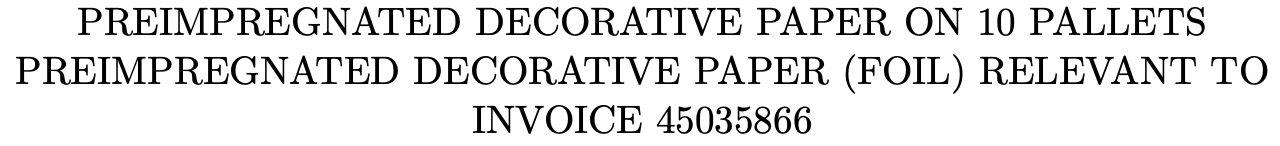
\includegraphics[width=1\textwidth]{bol1.png}
    \caption{An example of a text description, taken from the Bills of Lading summaries data set. Note that the quantity and the invoice are mentioned, and that the main description (preimpregnated decorative paper) is repeated.}
    \label{fig:eg BOL}
\end{figure}

Lastly, some of the product descriptions contain a HTS code, which is a ten- digit code that corresponds to a US-specific extension of the Harmonized system. This could be a serious problem for the validity of our approach, as any classifier could simply learn to associate these with a HS label. In order to mitigate leakage via these we remove any word that only contains digits and is longer than six digits.

\subsection{Atos Data Set}
This data set was collected in collaboration with a customs authority Atos has partnered with. The data set includes 5,457,325 descriptions of goods and their corresponding HS label, up to a HS-8 definition. These descriptions were collected from electronic administrative intake forms as they were submitted to the customs authority between 2015 and 2017. \\
The HS label data is assumed to have been corrected by the customs authority and the descriptions are in general, of high quality. In total the data set contains 5061 unique HS-8 labels, which are aggregated into 96 HS-2 labels and 1207 HS-4 labels. The number of unique goods descriptions in the data set is quite large: 3,108,080 (57{\%}) text descriptions appear only once in the data set. The average “sentence” length is quite small: the mean number of tokens encountered per description is 8.05, and the median value observed is 7. The most frequent token count however, is just three tokens, with the next largest group being descriptions that are just two tokens, as illustrated below.

\begin{figure}[th]
    \centering
    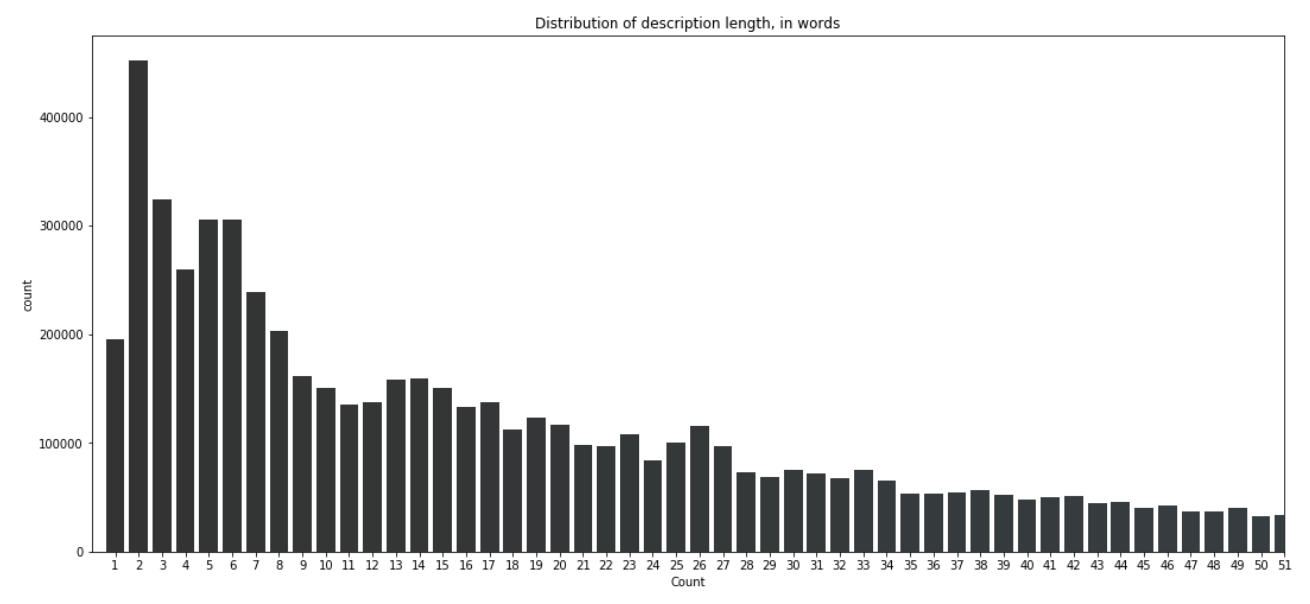
\includegraphics[width=0.8\textwidth]{BOL2.png}
    \caption{The distribution of description lengths in the Bills of Lading from 2017 data set. The counts shown are the number of words in the descriptions. The counts notable peak at 2 tokens.}
    \label{fig:Bol2}
\end{figure}

\begin{figure}[th]
    \centering
    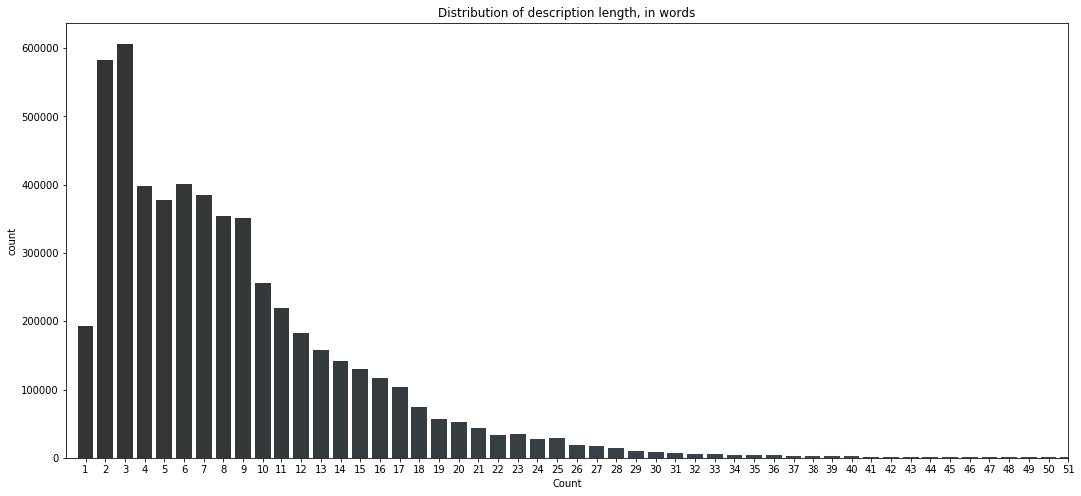
\includegraphics[width=0.8\textwidth]{data.jpg}
    \caption{The distribution of description lengths in the data set. The counts shown are the number of words in the descriptions}
    \label{fig:Data}
\end{figure}

There is a significant imbalance in the class distribution, with the smallest class, 43 (Furskins and artificial fur; manufactures thereof), being composed of only 47 items while the largest class, 87 (Vehicles other than railway or tramway rolling-stock, and parts and accessories thereof), accounts for 953,291 data points (17.5{\%} of all data). As such, there is not just a skewed distribution with regards to overall description length, but also in the class frequency distribution.


\textbf{Exemples}
\\

The data set is a company-specific data set and as such will not be released to the public domain with this thesis. I have therefore opted to include comprehensive lists of the amount of data points per HS-2 code and the descriptions of each HS-2 chapter to the appendix to this thesis.\\
\\
Table 3.1 directly illustrates some of the difficulties encountered with this data set. There are multiple items (item number 2, 3, and 4) that are essentially spare parts for some kind of machine: yet, these fall under three distinct chapters. Another salient feature of is the brevity of these text samples: an item such as ”handbags” is just one word. “Spice mixed” or “new drain” is similarly just two tokens. This serves to further illustrate the low information that can be gathered from these texts. Thirdly, some of these texts include potential valuable keywords such as “New” and “In Transit”.



\begin{center}
    \begin{tabular}{ll} \hline
HS-6 Code & Description  \\ \hline
271019 & GASOIL IN TRANSIT TO SOUTH SUDAN.TRUCK \\
842123 & NEW ATLAS COPCO AIR COMPRESSOR \\
& SPARE PARTS : PREVENTIVE MAINTENANCE KIT / \\
& SERVICE KIT : ORIGIN BELGIUM\\
854370 & NEW DRAIN\\
340319 & NEW OIL PISTON\\
420222 & HANDBAGS\\
091091 & SPICE MIXED\\
121190 & BASIL SEEDS (TAKMARIYA)\\ \hline
	\end{tabular}
\end{center}
{\textit{Table 3.1: Some descriptions and their corresponding HS-6 code from the data set. 
The descriptions are representative in the shortness of descriptions encountered in the data set.}} \\


\section{Pre-Procession}

For the data sets under consideration I perform a number of steps to pre-process the data. I first obtain a format of one description per line. 
I then replace diacritics with their unaccented form and convert the text to lowercase UTF-8. I preserve hyphens, but otherwise have a rather strict removal policy: I only keep alpha-numeric content, including spaces. However, extra white space is also removed, as words will be tokenized using the remaining spaces. However, I do not correct for spelling mistakes (such as "dinning" instead of "dining") which are frequent with data entered by human. I do also not remove stop words, or employ a stemming or lemmatization strategy. 
Lastly, I do not group common phrases together to make them appear in the data as one token (such as "new{\_}york" instead of "new york"). I also do not perform any part-of-speech (POS) tagging, syntactic dependency parsing, or named entity recognition (NER).
\\

The Netherlands team and I have not been able to find a curated data set in our domain of harmonized code classification to establish a benchmark. On a high level, the data sets we have found meet our goal of short text description. Of the two, the public Bills of Lading 2017 data set contains longer descriptions and is noisier. The Atos data set contains many shorter descriptions and can be assumed to be corrected, but it is not in the public domain. In order to allow for comparison, we will compare classification approaches on both data sets. Table 4.2 shows the number of data points in both data sets, along with the number of unique labels encountered at both levels of distinction.

\begin{center}
    \begin{tabular}{lrrr} \hline
Data Sets & Number of Samples & HS-2 Labels & HS-4 Labels\\ \hline
Bills of Lading & 7,641,625 & 99 & 1271\\
Atos & 5,457,325 & 99 & 1207\\ \hline
	\end{tabular}
\end{center}
{\textit{Table 3.1: Description of the data sets used in this project.}} \\

\chapter{Methods}
This section details the models developed and the methodology I followed.
\section{Tokenization for BERT}
\section{Fine-tuning}
